\begin{preface}
Computers are logic in action. Literally.
Computer components are realizations of formulas in logic,
and when activated by Boolean signals, those components
compute the value of the formula that they actualize.
Software too is an exhibit in logic.
A software component is a specification in a formal language
with underpinnings in logic,
and some software components
are, literally, algebraic formulas.
Big formulas, but formulas nevertheless.

Therefore, people studying computer science
benefit from studying logic, and
most computer science students
are exposed to logic in their education.
Often this exposure comes
in the form of a few lectures and a problem set or two
in a discrete math course. Applications of logic that
students see usually have more to do with traditional mathematics
than with computer science. Even when the course
is ``discrete math for computer science,'' the computer science
part often has more to do with writing programs to solve problems
in traditional mathematics than it has to do with
concepts in computer science.
We think computer science students will
benefit from a substantially more extensive and rigorous
exposure to logic and to seeing many applications of
logic in their chosen field of study.
All the examples in this text arise from issues in computer science.

This book focuses directly on central themes
in computer science.
It frames the discussion in terms of logic,
and it applies logic to problems in the domain of computer science.
Hardware components, software components,
testing and verification, and analysis of algorithms
are some examples.
Instead of illustrating mathematical induction by proving
that a formula represents the sum of a sequence of numbers,
we begin with an inductive proof of an important property of
a software component that concatenates lists,
and we proceed to verify properties of
many other software and hardware components.
It's the same old mathematical induction but presented
in the context of topics that interest
students of computer science.
The logic of induction is at the forefront,
unobscured by tricks in numeric algebra
that many exercises on induction require in
discussions grounded in topics
of particular interest to mathematicians.

We hope that readers will be inclined
to devote substantial effort, on the order
of what it takes to absorb a few dozen fifty-minute
lectures at the college level,
to understand some important problems in computer science and
to pursue solutions to many of those problems through formal reasoning.
Formalism is a watchword in this presentation, even to the
point of using the mechanized logic of a partially automated proof engine,
ACL2, that checks proofs to the last detail and can sometimes
bridge, on its own, gaps that traditional mathematical
proofs, even rigorous ones, leave open.

The text employs three formal notations:
traditional algebraic formulas of propositional and predicate logic
(and numeric algebra, occasionally),
digital circuit diagrams, and ACL2, which is syntactically
like Lisp, the programming language, but it is embedded
in a mechanized logic that assists in producing
formal proofs in first-order logic.
ACL2 serves as a mathematical notation, and all
of the material can be understood in terms of
traditional, paper-and-pencil reasoning
without putting formal models
through their paces on a computer system.
For readers who want to see formalization
in action, the text presents examples using
Proof Pad, a lightweight ACL2 environment.
ACL2 experts use emacs or the ACL2 Sedan
as their interface, and readers of this text can
use those tools if they prefer, but the text
illustrates the process in the Proof Pad framework,
which in our experience puts a low burden on novices.
In any case, Proof Pad will be adequate to support
study with this text.

We chose ACL2 as the proof engine for this work
because in our judgment it provides a more accessible
introduction to mechanized formalism than any other
available tool. We do not anticipate that any
reader will become an accomplished ACL2 user,
much less an ACL2 expert. We bring ACL2 into the discussion
to show how logic, including mechanized logic,
can benefit practicing software and hardware engineers.
Readers who want to realize those benefits in
large-scale projects will need to learn a lot more
about ACL2 or another mechanized logic than they
will glean from this introduction.
In former years, we presented logic in the classroom
without a mechanized logic, but we found through experience
that most students are more comfortable and motivated
when formal methods are backed up by tools
that check proofs and help
push through details.

Logic is the central topic of the text but not the only topic.
Readers interested in the broad outlines of computer science
will find material useful in that pursuit.
The text can provide a basis for a serious introduction
to computer science concepts, both for computer science students
and for students in other fields who want to know
what computer science is about.
Earlier versions of the text have been used many times
by the authors and other instructors
as the primary text in two types of courses: logic for computer science
and introduction to computer science for both computer science students
and students in other disciplines.
It has also been used as a supplementary
text in discrete math courses for computer science students.
The text has served well in all three realms.

There are no prerequisites beyond college prep, high school math.
Even less, really.
High school algebra is helpful,
but no geometry, trigonometry, or calculus is needed.
Programming experience is not a prerequisite either, and
the equation-based approach that informs this presentation can
help level the playing ground between people
with programming experience and those without it.
Students whose goal is to certify that they already
know the material are surprised to find that they don't,
whereas those who arrive with less background tend
to invest the necessary effort from the outset.

The required learning is far from easy.
Successful students will have to do a lot of hard thinking
to work their way through a few dozen exercises,
and they will surely need to do a few dozen exercises to grasp the concepts.
Reading alone won't be enough.
Exercises in the text (over 180 in all) afford students with opportunities
for problem solving.
Fortunately, the work pays off, both in terms of immediate satisfaction
and in the long term, if the testimonies of former students are a
reliable measure.
We hope readers will take some pleasure in working their way through
the book, and that they will find what they learn
edifying as they go on to other projects.

\vspace{0.5cm}
{\parindent0pt
\textbf{Prerequisite Knowledge and Chapter Dependencies}.
\label{ch:roadmap}
Equations provide a foundation
for rigorous, formal methods throughout the presentation.
Readers will need to understand equations at a level
typically acquired in high school algebra, but they will need
no other prerequisite knowledge.
Instructors, on the other hand, will find
a solid footing in equation-based programming advantageous.
Chapters on the practice of computation are more descriptive than rigorous.
These topics can be woven into the sequence at any point
and can usefully slow the pace of introduction
of challenging concepts in equations and reasoning.
The following diagram elucidates some possible
paths through the material.}
\\ %%\vspace{5mm}\\

\label{diagram:roadmap}
\begin{center}
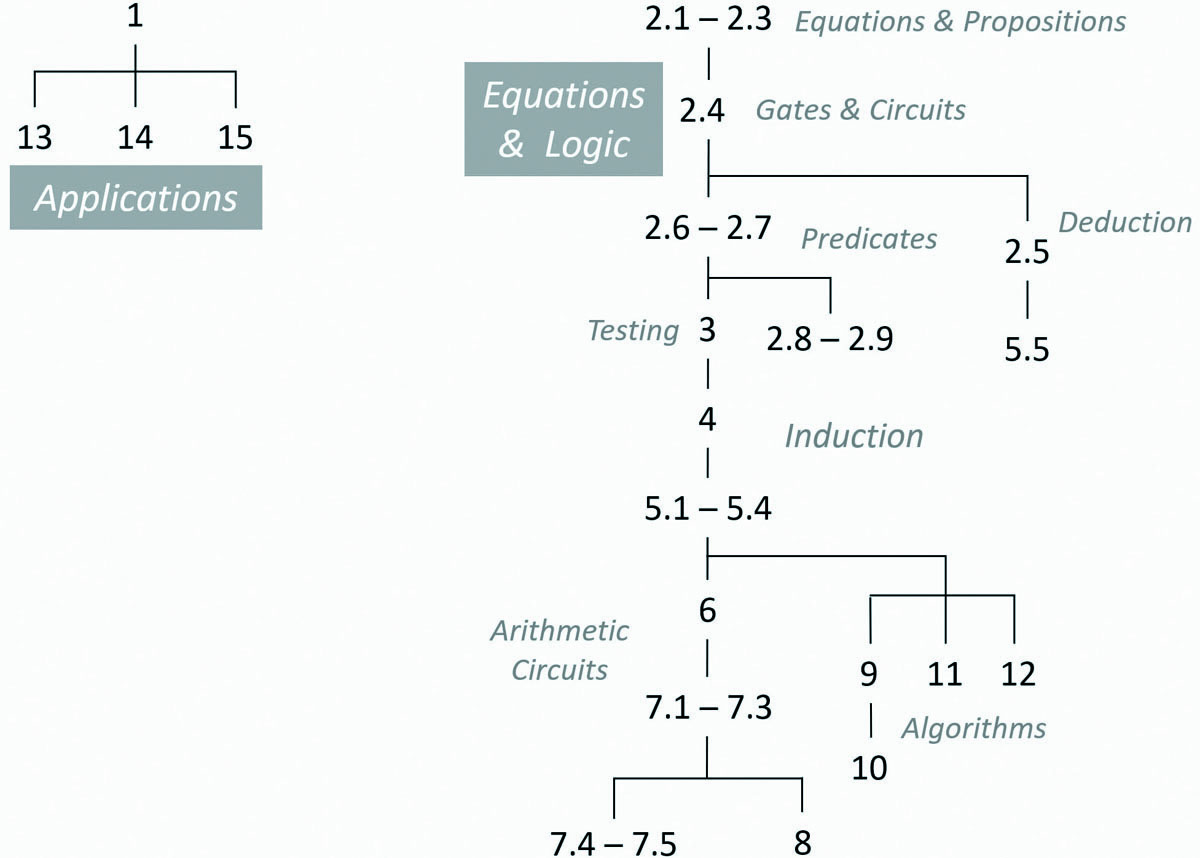
\includegraphics[scale=1]{images-cmyk/roadmap-cmyk.jpg} %% was: scale=0.23
\end{center}

\clearpage
{\parindent0pt
\textbf{Acknowledgments}.
\label{ch:Acknowledgements}
The authors would like to thank Caleb Eggensperger for developing
the Proof Pad environment that has eased many students
through early experiences with mechanized logic.
Carl Eastland, Dale Vaillancourt, and Matthias Felleisen
built an ACL2 environment that one of the authors relied on
for many course offerings and which
included DoubleCheck, the predicate-based, automated testing facility
based on ideas in QuickCheck, the grandaddy
of such tools invented by John Hughes and Koen Claessen,
that was later incorporated into Proof Pad.
We thank them for their pioneering work.
Qi Cheng used prototype versions of the text
in applied logic courses and
suggested improvements that made it a better book.
The authors also want to credit the students,
numbering more than a thousand,
who applied themselves to early versions of the
text and provided their feedback. Thank you, every one.}

\author{Rex Page and Ruben Gamboa}
\date{January, 2018}
\end{preface}
